\documentclass[compress]{beamer}
\usepackage{default}
\usepackage{graphicx}
\usepackage{amsfonts}
\usepackage{amssymb}
\usepackage{amsmath}
\usepackage[brazil]{babel}
\usepackage[utf8]{inputenc}
\usetheme{Szeged}
\usecolortheme{whale}

\title{Registo de Imagens\\Algoritmo Demons}
\author{Thiago de Gouveia Nunes}
\date{}

\begin{document}
\graphicspath{ {itk/}{rotacao/}{sobel/} }
\frame{\titlepage}

\section{Comparação com ITK}

\begin{frame}
  Comparação com os resultados obtidos pela ITK.
\end{frame}

\begin{frame}
  \begin{picture}(320,250)
  \put(25,10){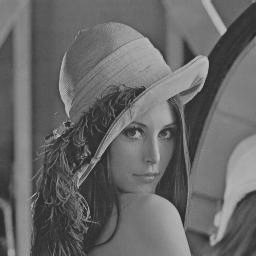
\includegraphics[scale=0.9]{lenaStatic.png}}
  \put(25,242){\begin{minipage}[t]{\linewidth}
  {Imagem de referência}
  \end{minipage}}
  \end{picture}
\end{frame}

\begin{frame}
  \begin{picture}(320,250)
  \put(25,10){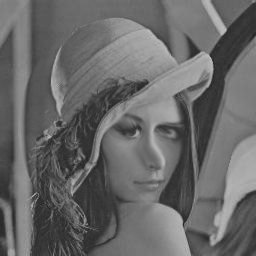
\includegraphics[scale=0.9]{lenaMoving.png}}
  \put(25,242){\begin{minipage}[t]{\linewidth}
  {Imagem que será registrada pelo demons}
  \end{minipage}}
  \end{picture}
\end{frame}

\begin{frame}
  \begin{picture}(320,250)
    \put(25,10){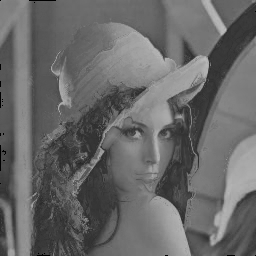
\includegraphics[scale=0.9]{itk-sym-lena.png}}
    \put(25,242){\begin{minipage}[t]{\linewidth}
    {Resultado obtido pela ITK}
    \end{minipage}}
  \end{picture}
\end{frame}

\begin{frame}
  \begin{picture}(320,250)
    \put(25,10){
\includegraphics[scale=0.9]{lenasymmetric.png}}
    \put(25,242){\begin{minipage}[t]{\linewidth}
    {Resultado obtido pelo demons simétrico.}
    \end{minipage}}
  \end{picture}
\end{frame}

\begin{frame}
  \begin{picture}(320,250)
    \put(25,10){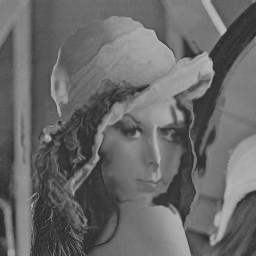
\includegraphics[scale=0.9]{lenaasymmetric.png}}
    \put(25,242){\begin{minipage}[t]{\linewidth}
    {Resultado obtido pelo demons asimétrico.}
    \end{minipage}}
  \end{picture}
\end{frame}

\begin{frame}
  \begin{picture}(320,250)
    \put(-5,140){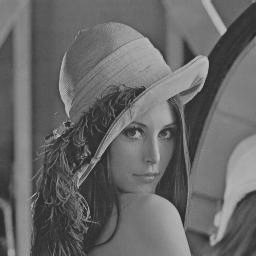
\includegraphics[scale=0.4]{lenaStatic.png}}
    \put(-5,130){\begin{minipage}[t]{0.4\linewidth}{Referência}\end{minipage}}
    \put(100,140){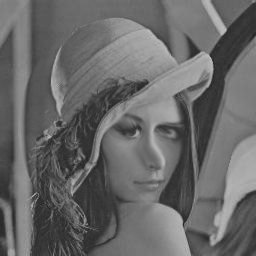
\includegraphics[scale=0.4]{lenaMoving.png}}
    \put(100,130){\begin{minipage}[t]{0.4\linewidth}{Movel}\end{minipage}}
    \put(205,140){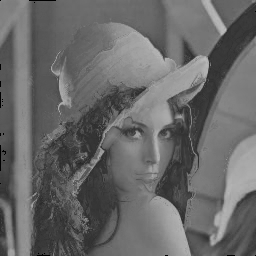
\includegraphics[scale=0.4]{itk-sym-lena.png}}
    \put(205,130){\begin{minipage}[t]{0.4\linewidth}{Resultado ITK}\end{minipage}}
    \put(35,20){
\includegraphics[scale=0.4]{lenasymmetric.png}}
    \put(35,10){\begin{minipage}[t]{0.4\linewidth}{Simétrico}\end{minipage}}
    \put(140,20){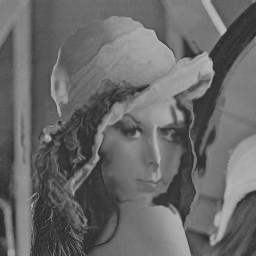
\includegraphics[scale=0.4]{lenaasymmetric.png}}  
    \put(140,10){\begin{minipage}[t]{0.4\linewidth}{Asimétrico}\end{minipage}}
  \end{picture}
\end{frame}

\section{Rotação}

\begin{frame}
  Resultados do demons variando a rotação de um quadrado.
\end{frame}

\begin{frame}
  \begin{picture}(320,250)
    \put(25,10){
\includegraphics[scale=0.9]{quadradoStatic.png}}
    \put(25,242){\begin{minipage}[t]{\linewidth}
    {Imagem de referência}
    \end{minipage}}
  \end{picture}
\end{frame}

\begin{frame}
  \begin{picture}(320,250)
    \put(25,10){
\includegraphics[scale=0.9]{moving5.png}}
    \put(25,242){\begin{minipage}[t]{\linewidth}
    {Imagem referência rotacionada em 5 graus}
    \end{minipage}}
  \end{picture}
\end{frame}

\begin{frame}
  \begin{picture}(320,250)
    \put(25,10){
\includegraphics[scale=0.9]{quadrado5symmetric.png}}
    \put(25,242){\begin{minipage}[t]{\linewidth}
    {Resultado da rotação em 5}
    \end{minipage}}
  \end{picture}
\end{frame}

\begin{frame}
  \begin{picture}(320,250)
    \put(25,10){
\includegraphics[scale=0.9]{moving15.png}}
    \put(25,242){\begin{minipage}[t]{\linewidth}
    {Imagem referência rotacionada em 15 graus}
    \end{minipage}}
  \end{picture}
\end{frame}

\begin{frame}
  \begin{picture}(320,250)
    \put(25,10){
\includegraphics[scale=0.9]{quadrado15symmetric.png}}
    \put(25,242){\begin{minipage}[t]{\linewidth}
    {Resultado da rotação em 15}
    \end{minipage}}
  \end{picture}
\end{frame}

\begin{frame}
  \begin{picture}(320,250)
    \put(25,10){
\includegraphics[scale=0.9]{moving30.png}}
    \put(25,242){\begin{minipage}[t]{\linewidth}
    {Imagem referência rotacionada em 30 graus}
    \end{minipage}}
  \end{picture}
\end{frame}

\begin{frame}
  \begin{picture}(320,250)
    \put(25,10){
\includegraphics[scale=0.9]{quadrado30symmetric.png}}
    \put(25,242){\begin{minipage}[t]{\linewidth}
    {Resultado da rotação em 30}
    \end{minipage}}
  \end{picture}
\end{frame}

\begin{frame}
  \begin{picture}(320,250)
    \put(25,10){
\includegraphics[scale=0.9]{moving45.png}}
    \put(25,242){\begin{minipage}[t]{\linewidth}
    {Imagem referência rotacionada em 45 graus}
    \end{minipage}}
  \end{picture}
\end{frame}

\begin{frame}
  \begin{picture}(320,250)
    \put(25,10){
\includegraphics[scale=0.9]{quadrado45symmetric.png}}
    \put(25,242){\begin{minipage}[t]{\linewidth}
    {Resultado da rotação em 45}
    \end{minipage}}
  \end{picture}
\end{frame}

\begin{frame}
  \begin{picture}(320,250)
    \put(-5,140){
\includegraphics[scale=0.4]{quadradoStatic.png}}
    \put(-5,130){\begin{minipage}[t]{0.4\linewidth}{Referência}\end{minipage}}
    \put(100,140){
\includegraphics[scale=0.4]{quadrado5symmetric.png}}
    \put(100,130){\begin{minipage}[t]{0.4\linewidth}{5 graus}\end{minipage}}
    \put(205,140){
\includegraphics[scale=0.4]{quadrado15symmetric.png}}
    \put(205,130){\begin{minipage}[t]{0.4\linewidth}{15 graus}\end{minipage}}
    \put(35,20){
\includegraphics[scale=0.4]{quadrado30symmetric.png}}
    \put(35,10){\begin{minipage}[t]{0.4\linewidth}{30 graus}\end{minipage}}
    \put(140,20){
\includegraphics[scale=0.4]{quadrado45symmetric.png}}  
    \put(140,10){\begin{minipage}[t]{0.4\linewidth}{45 graus}\end{minipage}}
  \end{picture}
\end{frame}

\section{Gradientes}

\begin{frame}
  Comparação entre a utilização do filtro Sobel para o cálculo do gradiente e o gradiente básico.
\end{frame}

\end{document}
